\documentclass[12pt]{article}
\usepackage{amsmath,amsthm,amssymb}
\usepackage{geometry}
\usepackage{makeidx}
\usepackage{graphicx}
\usepackage{color}
\usepackage[usenames,dvipsnames]{xcolor}
\usepackage{tikz}
\usepackage{xfrac}
\usepackage{array}
\usepackage{color}
\usepackage{listings}
\usepackage{bbm}
\lstset{ %
language=C++,
basicstyle=\footnotesize,
numbers=left,
numberstyle=\footnotesize,
stepnumber=1,
numbersep=5pt,
backgroundcolor=\color{white},
showspaces=false,% show spaces adding particular underscores
showstringspaces=false,% underline spaces within strings
showtabs=false,% show tabs within strings adding particular underscores
tabsize=2,% sets default tabsize to 2 spaces
captionpos=b,% sets the caption-position to bottom
breaklines=true,% sets automatic line breaking
breakatwhitespace=false,
escapeinside={\%*}{*)}          % if you want to add a comment within your code
}
\usepackage{xstring}

\usepackage[english,greek]{babel}
\usepackage[utf8x]{inputenc}
%\usepackage{ucs}

\usepackage{enumerate}
\usepackage{enumitem}
\setlist{nolistsep}
\usepackage{hyperref}
\hypersetup{colorlinks=true,linkcolor=MidnightBlue}

\newcommand\en[1]{\latintext #1\greektext}
\newcommand\m[1]{\mbox{$\displaystyle #1 $}}
\newcommand\ul[1]{\emph{#1}}
\newcommand\bigOh{\mathcal{O}}
\newcommand\nospace{\hspace*{-0.5em}}

\renewcommand{\thefootnote}{*}

\newenvironment{n_enum}{
\begin{enumerate}[label=(\arabic{*})]
  \setlength{\itemsep}{0pt}
  \setlength{\parskip}{0pt}
  \setlength{\parsep}{0pt}
}{\end{enumerate}}

\newenvironment{i_enum}{
\begin{enumerate}[label=(\roman{*})]
  \setlength{\itemsep}{0pt}
  \setlength{\parskip}{0pt}
  \setlength{\parsep}{0pt}
}{\end{enumerate}}

\newenvironment{a_enum}{
\begin{enumerate}[label=(\alph{*})]
  \setlength{\itemsep}{0pt}
  \setlength{\parskip}{0pt}
  \setlength{\parsep}{0pt}
}{\end{enumerate}}

\newenvironment{b_item}{
\begin{itemize}
  \setlength{\itemsep}{0pt}
  \setlength{\parskip}{0pt}
  \setlength{\parsep}{0pt}
}{\end{itemize}}

\newcommand{\HRule}{\rule{\linewidth}{0.1mm}}

\begin{document}
\begin{center}
{\bf Αλγόριθμοι και πολυπλοκότητα}\\
2η Σειρά Γραπτών ασκήσεων
\end{center}
Χειμερινό Εξάμηνο 2013-2014 \hfill Μπογιόκας Δημήτριος - ΜΠΛΑ
\HRule\\
{\bf Άσκηση 1}(α) Το πρόβλημα λύνεται με τον παρακάτω άπληστο αλγόριθμο. Θεωρώ τα $n$ αιτήματα ταξινομημένα ως προς τα $f_i$, σε αύξουσα σειρά. Αρχικά θεωρώ ότι κανένα μάθημα δεν γίνεται στις αίθουσες. Στη συνέχεια, με τη σειρά, για κάθε $i$ ελέγχω αν το μάθημα $i$ μπορεί να γίνει σε κάποια αίθουσα (σύμφωνα με αυτά που έχω αποφασίσει μέχρι το προηγούμενο βήμα) και αν ναι, ανάμεσα σε αυτές που τη χρονική στιγμή $s_i$ είναι άδειες, επιλέγω εκείνη που μέχρι το προηγούμενο βήμα αργεί περισσότερο να αδειάσει (ελαχιστοποιώ την ώρα που κάθε αίθουσα μένει άδεια) και αποφασίζω ότι το μάθημα $i$ θα γίνει σε αυτή. Αν δεν υπάρχει άδεια αίθουσα τη στιγμή $s_i$ αποφασίζω ότι το μάθημα δε θα γίνει. Ο αλγόριθμος υλοποιημένος σε \en{C++} είναι:
\latintext\begin{lstlisting}
[...] //headers
int n,k;
int room[n+1]; //final room for every i, 0 stands for no room
int last[k+1]; //f_i of the last lesson programmed to be accomplished in room s, for every s
int request[n+1][2]; //request[i][0]=s_i, request[i][1]=f_i

void greedy(int i) {
  int mins=0;
  int mind=INT_MAX;
  for(int s=1;s<=k;s++) {
    if(request[i][0]>=last[s]&&mind>request[i][0]-last[s]) {
      mins=s;
      mind=request[i][0]-last[s];
    }
  }
  if(mins>0) {
    last[mins]=request[i][1];
    room[i]=mins;
  }
  if(i<n) greedy(i+1);
}

int main() {
[...] //input, sorting
  greedy(1);
[...] //output
  return 0;
}
\end{lstlisting}\greektext
Για να δείξω την ορθότητα, υποθέτω μία βέλτιστη λύση που ταυτίζεται για τα αιτήματα $1,\ldots,i-1$ με τη λύση που δίνει ο παραπάνω αλγόριθμος και διαφέρει από το αίτημα $i$ και μετά. Θα δείξω ότι υπάρχει μια διαφορετική βέλτιστη λύση που να ταυτίζεται με τη λύση του παραπάνω αλγορίθμου για τα αιτήματα $1,\ldots,i$ (υποθέτω πάλι ότι τα αιτήματα διατάσσονται κατά αύξουσα σειρά ως προς τα $f_i$). Πρέπει να εξετάσω τις ακόλουθες 3 περιπτώσεις:
\begin{b_item}
\item Ο παραπάνω αλγόριθμος να μην ικανοποιεί το αίτημα $i$, ενώ η βέλτιστη λύση να το ικανοποιεί στην αίθουσα $s$. Αυτό δεν θα μπορούσε ποτέ να γίνει, από τη συνθήκη του παραπάνω αλγορίθμου να απορρίπτει ένα αίτημα μόνο εάν όλες οι αίθουσες είναι κατειλλημένες ήδη την ώρα $s_i$, από το βήμα $i-1$. Αφού οι λύσεις ταυτίζονται για $i-1$, δεν υπάρχει ελεύθερη αίθουσα να ικανοποιηθεί το αίτημα $i$ στη βέλτιστη λύση.
\item Ο παραπάνω αλγόριθμος να ικανοποιεί το αίτημα $i$ στη θέση $s$, ενώ η βέλτιστη λύση να μην το ικανοποιεί. Στην περίπτωση αυτή, έστω $j$ το πρώτο αίτημα που ικανοποιείται στην αίθουσα $i$ από τη χρονική στιγμή $s_i$ και μετά. Αφαιρώ το αίτημα $j$ από τη βέλτιστη λύση και το αντικαθιστώ με το αίτημα $i$. Ο συνολικός αριθμός των αιτημάτων που ικανοποιούνται δεν μεταβάλλεται, αφού $f_i\leq f_j$ και άρα όλα τα υπόλοιπα αιτήματα στην αίθουσα $s$ της βέλτιστης λύσης δεν επηρεάζονται. Άρα προκύπτει μια διαφορετική βέλτιστη λύση που ταυτίζεται από το αίτημα 1 έως και το $i$ με τη λύση που δίνει ο παραπάνω αλγόριθμος.
\item O παραπάνω αλγόριθμος να ικανοποιεί το αίτημα $i$ στην αίθουσα $s$, ενώ η βέλτιστη λύση να το ικανοποιεί στην αίθουσα $t$. Έστω $j$ το πρώτο αίτημα που ικανοποιείται στην αίθουσα $s$, στη βέλτιστη λύση, από τη χρονική στιγμή $s_i$ και μετά. Αντιμεταθέτω τότε, στη βέλτιστη λύση, όλα τα αιτήματα που ικανοποιούνται στην αίθουσα $s$ από το $j$ και μετά με όλα τα αιτήματα που ικανοποιούνται στην αίθουσα $t$ από το $i$ και μετά. Η συγκεκριμένη αντιμετάθεση μπορεί να γίνει. Πράγματι, το αίτημα $i$ (και κατά συνέπεια όλα τα επόμενα) ικανοποιείται στην αίθουσα $s$, αφού έτσι είναι η λύση που δίνει ο παραπάνω αλγόριθμος. Επίσης, το αίτημα $j$ (και κατά συνέπεια όλα τα επόμενα) ικανοποιείται στην αίθουσα $t$. Πράγματι, αν λαμβάνοντας υπ' όψιν μόνο τα πρώτα $i-1$ αιτήματα, οι αίθουσες $s$ και $t$ είναι κατειλλημένες έως τις χρονικές στιγμές $last_s$ και $last_t$ αντιστοίχως, τότε από την άπληστη επιλογή του παραπάνω αλγορίθμου, ισχύει $last_s\geq last_t\geq s_j$. Άρα, προκύπτει μια διαφορετική βέλτιστη λύση που ταυτίζεται από το αίτημα $1$ έως και το $i$ με τη λύση που δίνει ο παραπάνω αλγόριθμος.
\end{b_item}
Επίσης, κάθε βέλτιστη λύση ταυτίζεται με την παραπάνω με τετριμμένο τρόπο για $i=0$, άρα, επαγωγικά, υπάρχει κάποια βέλτιστη λύση που να ταυτίζεται με την παραπάνω για όλα τα αιτήματα από $1$ έως $n$, δηλαδή η παραπάνω λύση είναι βέλτιστη. Η πολυπλοκότητα του αλγορίθμου είναι $\Theta\left(nlogn+kn\right)$. Πράγματι, πέρα από την ταξινόμηση ($\Theta(nlogn)$) ο αλγόριθμος κάνει $k$ επαναλήψεις για κάθε μάθημα, για να βρει αν και σε ποιά αίθουσα θα το ικανοποιήσει.\\
\HRule\\
{\bf Άσκηση 1}(β) Προφανώς ο αλγόριθμος του (α) δεν εγγυάται τον υπολογισμό μιας βέλτιστης λύσης. π.χ. για $k=1$, $n=3$, $w_1=100, w_2=w_3=1$, $s_1=s_2=0, s_3=1$ και $f_1=f_3=2, f_2=1$ ο αλγόριθμος θα επιλέξει να γίνουν τα μαθήματα $2,3$, ενώ η βέλτιστη λύση είναι να γίνει το μάθημα $1$. Το παράδειγμα αυτό δείχνει μάλιστα ότι η βέλτιστη λύση μπορεί να απέχει αυθαίρετα πολύ από τη λύση που προκύπτει από τον παραπάνω αλγόριθμο, δηλαδή δεν είναι ούτε προσεγγιστικά καλός. Ένας αποδοτικός αλγόριθμος δυναμικού προγραμματισμού είναι ο εξής:\\
Θεωρώ τα αιτήματα ταξινομημένα σε αύξουσα σειρά ως προς τα $f_i$. Για κάθε επιλογή $k+1$ δεικτών $\left(i_1,\ldots,i_k,i_{k+1}\right)$, με $i_1<i_2<\cdots<i_{k+1}$ ορίζω συνάρτηση $b:\left\{0,1,\ldots,n\right\}^{k+1}\to\mathbb{N}$ που εκφράζει τη μερική βέλτιστη λύση του προβλήματος, όταν οι αίθουσες θεωρούνται άδειες από τις χρονικές στιγμές $f_{i_1},\ldots,f_{i_k}$ και μετά και έχω να αποφασίσω για τα μαθήματα $i_{k+1}+1,\ldots,n$ (Θεωρώ τη σταθερά $f_0$ με $f_0=0$, για να είναι καλά ορισμένη η συνάρτηση στην αρχική περίπτωση). Η αναδρομική σχέση που ισχύει για τη συνάρτηση $b$ είναι η ακόλουθη:
$$b\left(i_1,\ldots,i_k,i_{k+1}\right)=$$
$$\tiny=\left\{\begin{array}{lcl}
0&,&i_{k+1}=n\\
\max\left(\left\{b\left(i_1,\ldots,\widehat{i_m},\ldots,i_{k+1},i_{k+1}+1\right)+w_{i_{k+1}+1}:m\in\left\{1,\ldots,k\right\}\land f_{i_m}\leq s_{i_{k+1}+1}\right\}\cup\left\{b\left(i_1,\ldots,i_k,i_{k+1}+1\right)\right\}\right)&,&i_{k+1}<n\\
\end{array}\right.$$
όπου με $\widehat{i_m}$ συμβολίζω ότι το $i_m$ δεν περιέχεται στην $k+1$-άδα των αριθμών. Δηλαδή, η μερική βέλτιστη λύση ισούται με το μέγιστο ανάμεσα:
\begin{b_item}
\item στο να ικανοποιήσω το αίτημα $i_{k+1}+1$ σε κάποια άδεια αίθουσα (που είχε ικανοποιήσει πριν το αίτημα $i_m$), κερδίζοντας $w_{i_{k+1}+1}$ και όσο είναι το βέλτιστο με τις καινούριες συνθήκες (δηλαδή οι αίθουσες αδειάζουν όπως πριν, εκτός από αυτή που άδειαζε την χρονική στιγμή $f_{i_m}$ και τώρα αδειάζει την χρονική στιγμή $f_{i_{k+1}+1}$ και το μάθημα μέχρι το οποίο έχει τελειώσει η εξέταση να είναι το $i_{k+1}+1$), πάνω από όλα τα $m$ που ικανοποιούν τη συνθήκη η αντίστοιχη αίθουσα να είναι άδεια.
\item και στο να μην ικανοποιήσω το αίτημα $i_{k+1}+1$, κερδίζοντας όσο είναι το βελτιστο με τις καινούριες συνθήκες (δηλαδή οι αίθουσες να αδειάζουν όπως πριν και το μάθημα μέχρι το οποίο να έχει τελειώσει η εξέταση να είναι το $i_{k+1}+1$)
\end{b_item}
Στην παραπάνω αναδρομική σχέση δεν λαμβάνω υπ' όψιν συμμετρίες που προκύπτουν από μεταθέσεις των αιθουσών, αλλά τις αναδιατάσω κάθε φορά ώστε $f_{i_1}<f_{i_2}<\cdots<f_{i_k}$, χωρίς βλάβη της γενικότητας.\\
Προφανώς η λύση του προβλήματος είναι ο αριθμός $b\left(0,\ldots,0\right)$ δηλαδή όλες τις αίθουσες τις θεωρώ άδειες από τη χρονική στιγμή $f_0=0$ και τα μαθήματα που μένουν να εξεαστούν είναι τα $1,\ldots,n$.\\
Το πλήθος των διαφορετικών εισόδων της συνάτησης $b$ είναι το πλήθος του συνόλου $\left\{0,\ldots,n\right\}^{k+1}$, δηλαδή $\left(n+1\right)^{k+1}$ όπου με μία \en{top-bottom} υλοποίηση το πλήθος μειώνεται σε $\sum_{l=0}^{k+1}\binom{n}{k+1-l}$ ($l$ είναι το πλήθος των μηδενικών και στις υπόλοιπες $k+1-l$ θέσεις επιλέγω να βάλω έναν διαφορετικό αριθμό από το $\left\{1,\ldots,n\right\}$), που όμως είναι ασυμπτωτικά, για σταθερό $k$, ίσο με $\Theta\left(n^{k+1}\right)$. Σε κάθε υπολογισμό μίας τιμής της συνάρτησης, ο αλγόριθμος χρειάζεται $k+1$ επαναλήψεις για να βρει το μέγιστο ανάμεσα στις πιθανές τιμές που έχει υπολογίσει ήδη. Τελικά, σε κάθε περίπτωση, ο χρόνος που χρειάζεται ο αλγόριθμος είναι της τάξης $\bigOh\left(\left(k+1\right)\left(n+1\right)^{k+1}\right)$.\\
\HRule\\
{\bf Άσκηση 2} Το πρόβημα λύνεται με τον παρακάτω άπληστο αλγόριθμο. Θεωρώ τις Α κάρτες ταξινομημένες σε φθίνουσα σειρά ως προς τα $v_i$ και τις $B$ κάρτες ταξινομημένες σε αύξουσα σειρά ως προς τα $b_i$. Αρχικά θεωρώ ότι κανένα ταίριασμα δεν έχει γίνει. Στη συνέχεια, με τη σειρά για κάθε $i$ εξετάζω εάν η Α κάρτα $i$ μπορεί να κερδίσει κάποια ελεύθερη Β κάρτα (αν υπάρχει δηλαδή κάποιο $j$ που δεν έχω επιλέξει ήδη με $a_i>b_j$). Σε αυτή την περίπτωση επιλέγω το μέγιστο τέτοιο $j$. Διαφορετικά επιλέγω το μέγιστο $j$ που δεν έχω επιλέξει μέχρι τότε (και χάνω την κάρτα). Ο αλγόριθμος υλοποιημένος σε \en{C++} είναι:
\latintext\begin{lstlisting}
[...] //headers
int n;
int A[n+1][2]; //A[i][0]=a_i, A[i][1]=v_i
int B[n+1][2]; //B[i][0]=b_i, B[i][1]=j (the A card matched)
int score=0; //solution

int quickselectB(int x, int start, int end) {
  int med=(start+end)/2;
  if(start==end) return start;
  if(x<=B[med][0]) return quickselectB(x,start,med);
  else return quickselectB(x,med+1,end);
}

void greedy(int i) {
  int l=quickselectB(A[i][0], 1, n);
  if(l>0) {
    while(B[l][1]>0&&l>0) l--;
    if(l>0) {
      B[l][1]=i;
      score+=A[i][1];
    }
  }
  if(l==0) {
    int p=n;
    while(B[p][1]>0) p--;
    B[p][1]=i;
  }
  if(i<n) greedy(i+1);
}

int main() {
[...] //input, sorting
  greedy(1);
[...] //output
  return 0;
}
\end{lstlisting}\greektext
Για να δείξω την ορθότητα, υποθέτω μία βέλτιστη λύση που ταυτίζεται για τις Α κάρτες $1,\ldots,i-1$ με τη λύση που δίνει ο παραπάνω αλγόριθμος και διαφέρει από την Α κάρτα $i$ και μετά. Θα δείξω ότι υπάρχει μια διαφορετική βέλτιστη λύση που να ταυτίζεται με τη λύση του παραπάνω αλγορίθμου για τις Α κάρτες $1,\ldots,i$ (υποθέτω πάλι ότι οι Α κάρτες διατάσσονται κατά αύξουσα σειρά ως προς τα $v_i$ και ότι οι κάρτες Β διατάσσονται κατά αύξουσα σειρά ως προς τα $b_i$). Πρέπει να εξετάσω την εξής περίπτωση: Έστω ότι ο παραπάνω αλγόριθμος αντιστοιχίζει την $i$ Α κάρτα στην $j$ Β κάρτα, ενώ η βέλτιστη λύση αντιστοιχίζει την $i'>i$ Α κάρτα στην $j$ Β κάρτα και την $i$ κάρτα στην $j'$ Β κάρτα. Έστω $\psi$ η αξία όλων των κερδισμένων καρτών του βέλτιστου αλγορίθμου, εκτός από τις Α κάρτες $i$ και $i'$. Έτσι, η συνολική αξία των κερδισμένων καρτών στη βέλτιστη λύση είναι ίση με:
$$\mu=\psi+v_{i'}\mathbbm{1}_{\left(b_j,+\infty\right)}\left(a_{i'}\right)+v_i\mathbbm{1}_{\left(b_{j'},+\infty\right)}\left(a_i\right)$$
Αν αντικαταστήσω στην βέλτιστη λύση το ταίριασμα $(i,j'),(i',j)$ με το ταίριασμα $(i,j),(i',j')$, τότε η συνολική αξία των κερδισμένων καρτών θα είναι ίση με
$$\mu'=\psi+v_i\mathbbm{1}_{\left(b_j,+\infty\right)}\left(a_i\right)+v_{i'}\mathbbm{1}_{\left(b_{j'},+\infty\right)}\left(a_{i'}\right)$$
Έχουμε δηλαδή:
$$\mu'-\mu=v_i\mathbbm{1}_{\left(b_j,+\infty\right)}\left(a_i\right)+v_{i'}\mathbbm{1}_{\left(b_{j'},+\infty\right)}\left(a_{i'}\right)-v_{i'}\mathbbm{1}_{\left(b_j,+\infty\right)}\left(a_{i'}\right)-v_i\mathbbm{1}_{\left(b_{j'},+\infty\right)}\left(a_i\right)$$
Διακρίνω τις εξής δύο περιπτώσεις:
\begin{b_item}
\item$b_j<b_{j'}$. Σε αυτή την περίπτωση ισχύει $b_j<a_i\leq b_{j'}$. Πράγματι, αν $a_i\leq b_j$ τότε η κάρτα δε θα κερδιζόταν, οπότε ο αλγόριθμος θα επέλεγε το μέγιστο $b_j$ με αυτή την ιδιότητα, άτοπο. Ομοίως, αν $a_i>b_{j'}$ τότε η κάρτα θα κερδιζόταν, οπότε ο αλγόριθμος θα επέλεγε το μέγιστο $b_j$ με αυτή την ιδιότητα, επίσης άτοπο. Τέλος, λόγω της διάταξης έχουμε $v_i\geq v_{i'}$. Άρα ισχύει:
$$\begin{array}{rcl}\mu'-\mu
&=&v_i-v_{i'}\left(\mathbbm{1}_{\left(b_j,+\infty\right)}\left(a_{i'}\right)-\mathbbm{1}_{\left(b_{j'},+\infty\right)}\left(a_{i'}\right)\right)\\
&=&v_i-v_{i'}\mathbbm{1}_{\left(b_j,b_{j'}\right]}\left(a_{i'}\right)\\
&\geq&v_i-v_{i'}\\
&\geq&0\\
\end{array}$$
\item$b_{j'}\leq b_j$. Σε αυτή την περίπτωση ισχύει $a_i\notin\left(b_{j'},b_j\right]$. Πράγματι, αν $a_i>b_{j'}$ από την επιλογή του παραπάνω αλγορίθμου θα ισχύει και $a_i>b_j$ (αν υπάρχει τρόπος να κερδιθεί η κάρτα $i$, τότε κερδίζεται). Ομοίως με αντιθετοαντιστροφή, αν $a_i\leq b_j$ πάλι από την επιλογή του παραπάνω αλγορίθμου, θα ισχύει και $a_i\leq b_{j'}$ (αν η κάρτα $i$ δεν κερδιζει την $j$, τότε δεν υπάρχει κανένα $j'$ που να κερδίζει). Άρα ισχύει:
$$\begin{array}{rcl}\mu'-\mu
&=&v_{i'}\left(\mathbbm{1}_{\left(b_{j'},+\infty\right)}\left(a_{i'}\right)-\mathbbm{1}_{\left(b_j,+\infty\right)}\left(a_{i'}\right)\right)-v_i\left(\mathbbm{1}_{\left(b_{j'},+\infty\right)}\left(a_i\right)-\mathbbm{1}_{\left(b_j,+\infty\right)}\left(a_i\right)\right)\\
&=&v_{i'}\mathbbm{1}_{\left(b_{j'},b_j\right)}\left(a_{i'}\right)-v_i\mathbbm{1}_{\left(b_{j'},b_j\right)}\left(a_i\right)\\
&=&v_{i'}\mathbbm{1}_{\left(b_{j'},b_j\right)}\left(a_{i'}\right)\\
&\geq&0\\
\end{array}$$
\end{b_item}
Δηλαδή, σε κάθε περίπτωση ισχύει $\mu'\geq\mu$, άρα βρήκα μια βέλτιστη λύση που ταυτίζεται με την λύση του παραπάνω αλγόριθμου στις πρώτες $i$ Α κάρτες. Επίσης, για $i=0$ οι λύσεις ταυτίζονται με τετριμμένο τρόπο, άρα από επαγωγή η παραπάνω λύση είναι βέλτιστη. Ο χρόνος εκτέλεσης είναι $\bigOh\left(n^2\right)$. Πράγματι, πέρα από την ταξινόμηση, ο αλγόριθμος κάνει $n$ επαναλήψεις, όπου σε κάθε μία από αυτές κάνει $logn$ επαναλήψεις να βρει μια θέση του πίνακα Β, κοντά στην οποία αρχίζει να ψάχνει γραμμικά για κάποιο στοιχείο που δεν έχει χρησιμοποιηθεί. Δε θα χρειαστεί πάνω από $n$ επαναλήψεις σε αυτό το σημείο, εξ ου και το $\bigOh\left(n^2\right)$, αλλά το φράγμα δεν είναι ακριβές και ενδεχομένως με μια καλύτερη δομή δεδομένων να επιτυγχάνεται χρόνος $\Theta\left(nlogn\right)$.\\
\HRule\\
{\bf Άσκηση 3}(α) Ένα δέντρο χρωματίζεται με δύο χρώματα, σε γραμμικό χρόνο ως εξής: Χρωματίζουμε αυθαίρετα μία κορυφή με το χρώμα 1, στη συνέχεια τις κορυφές που απέχουν 1 από αυτή με το χρώμα 2, τις κορυφές που απέχουν 2 με το χρώμα 1 κ.ο.κ. Αποκλείεται να ενώνονται 2 κορυφές ίδιας απόστασης, γιατί τότε θα είχε κύκλο το γράφημα, το οποίο αποκλείεται επειδή είναι δέντρο. Στο ακόλουθο παράδειγμα:\\
\begin{center}
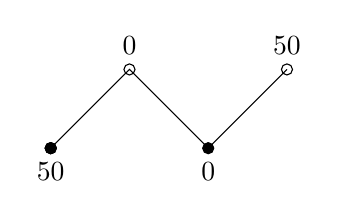
\begin{tikzpicture}
\foreach\x in {(0,0),(2,0),}
 \filldraw[black] \x circle (2pt);
\foreach\x in {(1,1),(3,1),}
 \draw[black] \x circle (2pt);
\draw (0,0)--(1,1)--(2,0)--(3,1);
\node at (0,-0.3) {\m{50}};
\node at (1,1.3) {\m{0}};
\node at (2,-0.3) {\m{0}};
\node at (3,1.3) {\m{50}};
\end{tikzpicture}
\end{center}
ο αλγόριθμος αυτός επιλέγει είτε τις μαύρες, είτε τις λευκές κουκίδες. Σε κάθε περίπτωση επιλέγει συνολικό βάρος ίσο με 50, ενώ θα μπορούσε να επιλέξει μόνο τις 2 ακραίες κορυφές και να έχει συνολικό βάρος ίσο με 100. Ο αλγόριθμος αυτός όμως θα επιστρέφει πάντα τουλάχιστον το 50\% του βέλτιστου συνολικού βάρους. Ένα παράδειγμα που το κάνει είναι το παραπάνω και η απόδειξη ότι ποτέ δε θα επιστρέψει λιγότερο από 50\% είναι η εξής: $w=\max\left\{w\left(I_0\right),w\left(I_1\right)\right\}\geq\frac{w\left(I_0\right)+w\left(I_1\right)}{2}=50\% w\left(V\left(T\right)\right)\geq 50\% w'$
όπου $w$ το αποτέλεσμα του αλγορίθμου και $w'$ το βέλτιστο συνολικό βάρος.\\
\HRule\\
{\bf Άσκηση 3}(β) Ένας δυναμικός αλγόριθμος που λύνει αυτό το πρόβλημα βασίζεται στις εξής αναδρομικές σχέσεις:
$$\begin{array}{>{\displaystyle}rc>{\displaystyle}l}
weight\left(T,v,-1\right)&=&\sum_{u\in N_T\left(v\right)}\max\left\{weight\left(C_u,u,1\right),weight\left(C_u,u,-1\right)\right\}\\
weight\left(T,v,1\right)&=&w\left(v\right)+\sum_{u\in N_T\left(v\right)}weight\left(C_u,u,-1\right)\\
\end{array}$$
όπου $N_T\left(v\right)$ η περιοχή του σημείου $v$ μέσα στο $T$ και $C_u$ η συνεκτική συνιστώσα του $T\setminus v$, που περιέχει το $u$. Επίσης το $\pm1$ ως τρίτη παράμετρος συμβολίζει το κατά πόσον η $v$ θα συμπεριληφθεί τελικά στη λύση.
Αν διαλέξω μια αρχική κορυφή, αυθαίρετα, ως ρίζα, η σχέση γράφεται διαφορετικά ως εξής:
$$\begin{array}{>{\displaystyle}rc>{\displaystyle}l}
weight\left(v,-1\right)&=&\sum_{\underset{u\neq parent(v)}{u\in N_T\left(v\right)}}\max\left\{weight\left(u,1\right),weight\left(u,-1\right)\right\}\\
weight\left(v,1\right)&=&w\left(v\right)+\sum_{\underset{u\neq parent(v)}{u\in N_T\left(v\right)}}weight\left(u,-1\right)\\
\end{array}$$
Όλες οι ενδιάμεσες τιμές της συνάρτησης αποθηκεύονται σε έναν πίνακα με $2$ γραμμές και $n$ στήλες. Κάθε στήλη αντιστοιχεί σε έναν κόμβο, η μία γραμμη στην μερική βέλτιστη λύση χωρίς τον κόμβο και η άλλη στην μερική βέλτιστη λύση με τον κόμβο.\\
Η δομή δεδομένων που θα χρησιμοποιήσω για την αποθήκευση του δέντρου είναι αυτή της λίστας από συνδεδεμένες λίστες, αφού το γράφημα είναι τόσο αραιό. Τελικά ο αλγόριθμος θα εξετάσει 2 φορές κάθε ακμή, δηλαδή τελικά θα χρειαστεί γραμμικό χρόνο. Ο αλγόριθμος αυτός (η \en{up-down} μορφή του) υλοποιημένος σε \en{C++} είναι:
\latintext\begin{lstlisting}
[...] //headers
struct node {
  node* prev;
  node* next;
  int name;
};
int n;
node N[n+1];
int w[n+1];
int dynweight[n+1][2];

int max(int x,int y) {
  if(x>y) return x;
  else return y;
}

int weight(node u,node v, bool sign) {
  int solution=0;
  node p=N[u.name];
  while(p.next!=NULL) {
    if(p.name!=v.name) {
      if(sign) {
        if(dynweight[p.next->name][0]==0) dynweight[p.next->name][0]=weight(*(p.next),u,!sign);
        solution+=dynweight[p.next->name][0];
      }
      else {
        if(dynweight[p.next->name][0]==0) dynweight[p.next->name][0]=weight(*(p.next),u,sign);
        if(dynweight[p.next->name][1]==0) dynweight[p.next->name][1]=weight(*(p.next),u,!sign);
        solution+=max(dynweight[p.next->name][0],dynweight[p.next->name][1]);
      }
    }
    p=*(p.next);
  }
  if(sign) solution+=w[u.name];
  return solution;
}

int main() {
[...] //input
  node foo={NULL,NULL,0};
  int final=max(weight(N[1],foo,true),weight(N[1],foo,false));
[...] //output
  return 0;
}\end{lstlisting}\greektext
Χωρίς βλάβη της γενικότητας θεωρώ ότι όλες οι κορυφές έχουν θετικό βάρος, οπότε αρχικοποιώ τον $dynweight[][]$ με μηδενικά που σημαίνουν «δεν έχει εξεταστεί η περίπτωση». Μια παραλλαγή του κώδικα ώστε να μην χάνει χρόνο σε μηδενικές τιμές θα ήταν να αρχικοποιήσω τον πίνακα με τιμές ίσες με $-1$.\\
\HRule\\
{\bf Άσκηση 4} Το πρόβλημα λύνεται με τον παρακάτω δυναμικό αλγόριθμο. Ορίζω την ακόλουθη ποσότητα (για τον πληθάριθμο ενός συνόλου $K$ χρησιμοποιώ τον συμβολισμό $\# K$, αντί για το $\left|K\right|$):
$$a_i\left(k\right)=\#\left\{S\subset N\setminus\left\{i\right\}:w\left(s\right)=k\right\}$$
για κάθε $i\in N$ και $k\in\left\{0,\ldots,w\left(N\right)\right\}$. Δηλαδή το πλήθος των συνασπισμών που δε συμμετέχει το κόμμα $i$ και συγκεντρώνουν ακριβώς $k$ έδρες. Προφανώς τότε, για το ζητούμενο $b_i$ ισχύει:
$$b_i=\sum_{k=Q-w_i}^{Q-1}a_i\left(k\right)$$
Αρκεί δηλαδή να κατασκευαστεί ένας πίνακας $n\times Q$ που θα αποθηκεύει κάθε $a_i\left(k\right)$ για $i\in N$ και $k\in\left\{0,\ldots,Q\right\}$. Τον πίνακα αυτόν τον κατασκευάζω ως εξής:
Έστω $M=\left(m_{ij}\right)_{1\leq i\leq n\ ,\ 0\leq j\leq Q-1}$ ένας πίνακας που αρχικοποιείται με $0$ σε κάθε του συντεταγμένη, εκτός από την πρώτη στήλη που αρχικοποιείται με $1$, δηλαδή $m_{i0}=1$ για κάθε $i$ και $m_{ij}=0$ για κάθε $i$ και κάθε $j>0$. Κατασκευάζω τον τελικό πίνακα σε $n$ διαδοχικά βήματα που κάθε βήμα μετασχηματίζει τον πίνακα $M$ στον πίνακα $M'=\left(m'_{ij}\right)$ που χρησιμοποιείται στο επόμενο βήμα. Στο $i$ βήμα ορίζω τα $m_{xy}'$ από την ακόλουθη σχέση:
$$m'_{xy}=\left\{\begin{array}{lcl}
m_{xy}&,&x=i\\
m_{xy}&,&x\neq i\land y<w_i\\
m_{xy}+m_{x\left(y-w_i\right)}&,&x\neq i\land y\geq w_i\\
\end{array}\right.$$
Δηλαδή:
\begin{b_item}
\item Η $i$ γραμμή μένει αναλλοίωτη, αφού σε αυτή τη γραμμή μετράω το πλήθος των συνασπισμών που δεν περιέχουν το $i$
\item Ένας συνασπισμός ανάμεσα στα κόμματα $\left\{1,\ldots,i\right\}$ έχει ακριβώς $k$ έδρες, είτε χωρίς το $i$ ($m_{xk}$ διαφορετικές επιλογές), είτε μαζί με το $i$ (όπου σε αυτή την περίπτωση υπάρχουν $m_{x\left(k-w_i\right)}$ επιλογές για τα υπόλοιπα κόμματα). Το συνολικό πλήθος επιλογών αντιστοιχεί στο άθροισμα των δύο αυτών αριθμών.
\end{b_item}
Μετά από το $i$-οστό βήμα, ο πίνακας περιγράφει τη μερική βέλτιστη λύση, λαμβάνοντας υπ' όψιν τα κόμματα $1$ έως $i$. Άρα, ο τελικός πίνακας, μετά το $n-$οστό βήμα έχει για στοιχεία $m_{xy}$ ακριβώς το πλήθος των διαφορετικών συνασπισμών που δε συμμετέχει το $x$ και έχουν $y$ έδρες συνολικά, δηλαδή το ζητούμενο $a_x\left(y\right)$. Ο πίνακας αυτός για να κατασκευαστεί χρειάστηκε $n$ επαναλήψεις που σε κάθε μία υπολογίζονται $nQ$ το πλήθος στοιχεία, άρα τελικά χρόνο $\bigOh\left(n^2Q\right)$. Στη συνέχεια υπολογίζω τα $n$ το πλήθος $b_i$ με $w_i$ επαναλήψεις το κάθε ένα, όπου $w_i\leq Q$. Τέλος υπολογίζω σε χρόνο γραμμικό το $\bar{b}=\sum_{i=1}^nb_i$ και το ζητούμενο $B_i=\frac{b_i}{\bar{b}}$. Δηλαδή συνολικά απαιτείται χρόνος $\bigOh\left(n^2Q\right)$.\\
Στην πραγματικότητα η κατασκευή αυτού του πίνακα δεν είναι απαραίτητη. Αυτό φαί\-νε\-ται από την εξής παρατήρηση: Αν κατασκευάσω τη γεννήτρια συνάρτηση της ακολουθίας της γραμμής $l$ στο βήμα $i-1$, έστω
$$G_l^{i-1}\left(x\right)=\sum_{y=0}^{Q-1}m_{ly}x^y$$
τότε η επαγωγική κατασκευή (αν $l\neq i$) περιγράφεται ακριβώς από τη σχέση:
$$G_l^i\left(x\right)=\left(1+x^{w_i}\right)G_l^{i-1}\left(x\right)$$
επίσης ισχύει $G_0\left(x\right)=1$. Μετά το $n$-οστό βήμα, για κάθε γραμμή θα ισχύει το εξής:
$$A_i\left(x\right)=\prod_{j\in N\setminus\left\{i\right\}}\left(1+x^{w_j}\right)$$
όπου έχω θέσει $A_i\left(x\right)=G_i^n\left(x\right)$. Για κάθε $A_i\left(x\right)$ κατασκευάζω δηλαδή μια γραμμή $i$ με τους συντελεστές του πολυωνύμου. Τα πολυώνυμα αυτά όμως τελικά δεν διαφέρουν πάρα πολύ μεταξύ τους, δηλαδή μπορώ να γράψω:
$$A_i\left(x\right)=\frac{\prod_{j\in N}\left(1+x^{w_j}\right)}{1+x^{w_i}}$$
Θέτοντας δηλαδή $A\left(x\right)=\prod_{j\in N}\left(1+x^{w_j}\right)$ και χρησιμοποιόντας το $A_i\left(x\right)=\sum_{j=0}^{Q-1}a_i\left(j\right)x^j$ έχω τη σχέση:
$$\sum_{j=0}^{Q-1}a_i\left(j\right)x^j=\frac{A\left(x\right)}{1+x^{w_i}}\qquad(1)$$
Έστω ότι $A\left(x\right)=\sum_{k=0}^{w\left(N\right)} v_kx^k$. Τους πρώτους $Q$ συντελεστές του πολυωνύμου αυτού μπορώ να τους προσδιορίσω με την μέθοδο που κατασκεύασα τον πρώτο πίνακα, χρησιμοποιόντας αυτή τη φορά έναν πίνακα $1\times Q$, σε χρόνο $\bigOh\left(nQ\right)$. Αρκεί τώρα να υπολογίσω τους συντελεστές $a_i\left(j\right)$ χωρίς να χρειαστεί να αποθηκεύσω κάτι άλλο. Σε αυτό το σημείο χρησιμοποιώ τη γνωστή ταυτότητα των γεννήτριων συναρτήσεων:
$$\frac{1}{1-x}=\sum_{s=0}^\infty x^s$$
Δηλαδή, η σχέση $(1)$ γίνεται:
$$\begin{array}{>{\displaystyle}rc>{\displaystyle}l}\sum_{j=0}^{Q-1}a_i\left(j\right)
&=&\frac{A\left(x\right)}{1-\left(-x^{w_i}\right)}\\
&=&\left(\sum_{s=0}^\infty\left(-1\right)^sx^{sw_i}\right)\left(\sum_{k=0}^{w\left(N\right)}v_kx^k\right)\\
\end{array}$$
και από τον κανόνα γινομένου των δυναμοσειρών έχουμε:
$$a_i\left(j\right)=\sum_{s=0}^{\left\lfloor\frac{j}{w_i}\right\rfloor}\left(-1\right)^sv_{j-w_is}$$
το παραπάνω ισχύει επειδή όλοι οι συντελεστές των $x^k$ για $k\not\equiv0\mod w_i$ είναι ίσοι με $0$ στην αριστερή δυναμοσειρά, άρα μένουν μόνο οι συντελεστές των $1,x^{w_i},x^{2w_i},\ldots$ που είναι $\pm1$. Δηλαδή ισχύει τελικά:
$$b_i=\sum_{k=Q-w_i}^{Q-1}\sum_{s=0}^{\left\lfloor\frac{k}{w_i}\right\rfloor}\left(-1\right)^sv_{k-w_is}$$
για το πλήθος $T_i$ των επαναλήψεων που χρειάζονται για τον υπολογισμό του κάθε $b_i$ ισχύει:
$$T_i=\sum_{k=Q-w_i}^{Q-1}\frac{k}{w_i}\leq\sum_{k=Q-w_i}^{Q-1}\frac{Q}{w_i}=w_i\frac{Q}{w_i}=Q$$
και καθώς τα $b_i$ είναι $n$ το πλήθος, συνολικά χρειαζόμαστε χρόνο $\bigOh\left(nQ\right)$. Μετά από αυτό ο αλγόριθμος συνεχίζει όπως πριν στον υπολογισμό του $\bar{b}$ και τελικά των $B_i$. Συνολικά ο αλγόριθμος χρειάζεται λοιπόν $\bigOh\left(nQ\right)$ χρόνο να υπολογίσει τους συντελεστές του $A\left(x\right)$, στη συνέχεια $\bigOh\left(nQ\right)$ χρόνο να υπολογίσει τα $b_i$ με το εναλλασόμενο άθροισμα και τελικά γραμμικό χρόνο για να υπολογίσει τα $B_i$, δηλαδή συνολικό χρόνο $\bigOh\left(nQ\right)$. Ένα πρόγραμμα που υλοποιεί τον παραπάνω αλγόριθμο σε \en{C++} είναι το ακόλουθο:
\latintext\begin{lstlisting}
[...] //headers
int N;
int Q;
int w[N+1];
int A[Q];
int b[N+1];
int barb;
double B[N+1];

void makeA() {
  A[0]=1;
  int B[Q];
  for(int i=1;i<=N;i++) {
    for(int j=0;j<Q;j++) B[j]=0;
    int k=0;
    while(k+w[i]<Q) {
      B[k+w[i]]=A[k];
      k++;
    }
    for(int j=0;j<Q;j++) A[j]+=B[j];
  }
}

void makeb() {
  for(int i=1;i<=N;i++) {
    for(int k=Q-w[i];k<Q;k++) {
      for(int s=0;s<=k/w[i];s++) {
        if(s%2==0) b[i]+=A[k-w[i]*s];
        else b[i]-=A[k-w[i]*s];
      }
    }
  }
}

void makebarb() {
  for(int i=1;i<=N;i++) barb+=b[i];
}

void makeB() {
  for(int i=1;i<=N;i++) B[i]=(double)b[i]/barb;
}

int main() {
[...] //input
  makeA();
  makeb();
  makebarb();
  makeB();
[...] //output
  return 0;
}
\end{lstlisting}\greektext
\HRule\\
{\bf Άσκηση 5} Ένας δυναμικός αλγόριθμος που λύνει το πρόβλημα βασίζεται στην παρακάτω αναδρομική σχέση:
$$\mathcal{E}\left(k\right)=\left\{\begin{array}{>{\displaystyle}lc>{\displaystyle}l}
\left(\prod_{i=1}^kp_i\right)k^4+\sum_{s=1}^k(1-p_s)\left(\prod_{i=s+1}^kp_i\right)\left(\mathcal{E}\left(s-1\right)+\left(k-s\right)^4\right)&,&k>0\\
0&,&k=0\\
\end{array}\right.$$
Ο αλγόριθμος γεμίζει δυναμικά δύο πίνακες: έναν $n\times n$ που στην $(i,j)$ θέση αποθηκεύει την τιμή $\prod_{l=i}^jp_l$, για να έχει ο αλγόριθμος πρόσβαση σε αυτά σε σταθερό χρόνο και τον βασικό πίνακα-γραμμή με τη μερική βέλτιστη λύση, που στην θέση $k$ αποθηκεύει την τιμή της παραπάνω συνάρτησης, δηλαδή ποιό είναι το αναμενόμενο κέρδος μέχρι και την ερώτηση $k$. Μια υλοποίηση του αλγορίθμου σε \en{C++} είναι η εξής:
\latintext\begin{lstlisting}
[...] //headers
int n;
double prob[n+1];
double prod[n+1][n+1];
double E[n+1];

double product(int i, int j) {
  if(i>j) return 1;
  if(prod[i][j]==0) {
    prod[i][j]=product(i,j-1)*prob[j];
  }
  return prod[i][j];
}  

double profit(int k) {
  if(k==0) return 0;
  else if(E[k]==0) {
    E[k]+=product(1,k)*pow(k,4);
    for(int s=1;s<=k;s++) {
      E[k]+=(1-prob[s])*product(s+1,k)*(profit(s-1)+pow(k-s,4));
    }
  }
  return E[k];
}

int main() {
[...] //input
  int solution=profit(n);
[...] //output
  return 0;
}
\end{lstlisting}\greektext
Ο αλγόριθμος χρειάζεται τετραγωνικό χρόνο, επειδή κάνει $k$ επαναλήψεις για κάθε $k$, ώστε να υπολογίσει το άθροισμα του αναδρομικού τύπου και επειδή ο πίνακας που αποθηκεύει τα γινόμενα, χρειάζεται και αυτός τετραγωνικό χρόνο για να δημιουργηθεί, αφού οι τιμές υπολογίζονται αναδρομικά με το αναδρομικό βήμα να χρειάζεται σταθερό χρόνο.
\end{document}
